\documentclass[a4paper, 12pt]{article}
\usepackage[margin=13mm]{geometry}
\usepackage{lmodern}
\usepackage{multicol}
\usepackage{titlesec}
\usepackage{graphicx}
\usepackage{caption}
\usepackage{booktabs}
\usepackage{amsmath}
\usepackage{microtype}
\graphicspath{{figures/}{../analysis/results/}}

\newcommand\textline[4][t]{%
  \par\smallskip\noindent\parbox[#1]{.333\textwidth}{\raggedright #2}%
  \parbox[#1]{.333\textwidth}{\centering #3}%
  \parbox[#1]{.333\textwidth}{\raggedleft #4}\par\smallskip%
}

\titleformat{\section}{\normalfont\large}{\thesection.}{1em}{}
\titleformat{\subsection}{}{\thesubsection.}{1em}{}
\titlespacing{\section}{0pt}{5pt}{3pt}
\setlength{\abovedisplayskip}{3pt}
\setlength{\columnsep}{5mm}
\captionsetup{font=footnotesize, skip=3pt}
\linespread{0.93}\selectfont
\renewcommand{\arraystretch}{0.95}

\begin{document}

\textline[t]{\,\,}{Preprint of graduation study}{Jul. 28, 2026}
\vspace{0.1\baselineskip}
\begin{flushright}
  \begin{tabular}{@{}ll@{}}
    Name:       & Adriel Imaran Santoso  \\
    Supervisor: & Prof. Koichi Hashimoto \\
  \end{tabular}
\end{flushright}
\begin{center}
  Title: Tactile-Feedback Teleoperation: Grip Force and Grasping Performance \\
  Across Haptic Actuator Types for Fragile and Deformable Objects
\end{center}
\vspace{0.2\baselineskip}
\begin{multicols}{2}

  \section{Introduction}

  When we pick up an egg, our fingertips tell us how hard we are squeezing, and we stop
  before it cracks. In \emph{teleoperation}, where an operator drives a robot from a
  distance and watches it on a screen, that sense is missing, so the operator can only guess
  whether the grip is too loose to hold the object or hard enough to break it. People plan
  grip force from what they feel rather than from what they see, so removing touch removes
  the signal that plan is built on [1].

  The usual fix is a \emph{haptic device}, something worn on the hand that reproduces a
  sensation on the skin, such as a vibration. The part making that sensation is the
  \emph{actuator}. Most work picks one actuator and asks only whether feedback beats no
  feedback [2], leaving the choice of actuator unexamined. We ask both questions at once.
  Does touch feedback help an operator grasp fragile and squishy objects, and does it matter
  which actuator delivers it? Twenty-two people each tried three conditions, vision only and
  two actuator types.

  \section{System}

  The setup has three parts, a PC, a two-fingered robot gripper, and a small microcontroller
  worn on the operator's hand. About 30 Hz, the PC measures the gap between the operator's
  thumb and index finger using a hand-tracking library. That gap tells the gripper how far to
  open, so pinching in the air closes the robot hand. The system also measures the robot's grip
  and sends that back to the operator.

  It also reads two \emph{vision-based touch sensors} [3] on the gripper's fingertips, each a
  soft gel pad with a camera looking at it from inside. When an object presses into
  the gel, the camera sees the dent and software turns the image into a map of how deeply
  each point is pressed in. We reduce that map to two numbers, the total dented volume (a
  stand-in for grip force, so forces below are in arbitrary units, a.u., not newtons) and the
  deepest point of the dent in millimetres. That depth becomes a 0-to-1 ``intensity'', where
  1 means as hard as the object should ever be squeezed, and goes over USB to the wearable
  device. For safety the gripper stops closing once the dent passes 1.0~mm.

  Both actuator types are driven by that same number, so any difference comes from the
  hardware, not the software. LRA stands for \emph{linear resonant actuators}, tiny motors
  that buzz along one axis, like a phone vibration but cleaner, worn at the base joints of
  the thumb and index finger. EM stands for \emph{electromagnetic latching actuators} [4],
  where a short pulse flips a small magnet between two positions and it stays there with no
  further power, moving only when pulsed rather than vibrating continuously. Ours sit on the
  thumb and index fingertips, with the original design's skin-poking pin replaced by a single
  magnet so it could tap continuously. Higher intensity means a stronger buzz for the LRA and
  faster taps for the EM. Both grow smoothly with pressure. They differ in technology and,
  because of their size, in where on the finger they fit.

  \section{Method}

  The experiment compared how the three conditions affected grasping performance. Each of the
  22 participants tried all three (vision only, LRA, EM) in a \emph{within-subjects} design, in
  which every person is their own comparison, so differences in natural dexterity drop out.
  Two object classes were used, fragile ones, which break suddenly if squeezed too hard, and
  deformable ones, which squash gradually. Each participant performed five grasps per condition
  and class, giving 660 trials. Vision only ran first for nearly everyone, with LRA and EM
  varied after it. That order was not fully balanced, which matters later (Section~5).

  From each recording we computed peak grip force (largest dented volume), peak dent depth,
  wasted squeezing (force added \emph{after} the dent stopped deepening, which gains
  nothing), force reversals after that point (tightening and loosening again, or hunting for
  the right force), and, for fragile objects, survival. Each participant's five trials were
  reduced to their median (middle value).

  A \emph{p-value} is the chance of seeing a difference this large if the conditions were
  really identical, and below .05 is conventionally called significant. We tested whether the
  three conditions differ at all (Friedman test), then compared them two at a time (Wilcoxon
  signed-rank test), raising the p-values to account for how many pairs were tested (Holm
  correction). LRA and EM also got an \emph{equivalence test}, which asks the reverse
  question, not whether they differ but whether they are close enough to call the same. After
  each condition participants rated their experience on 5-point scales (\emph{Likert} items,
  1 = worst, 5 = best), and finally chose the condition they preferred.

  \section{Results}

  \begin{center}
    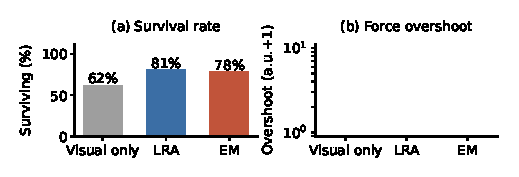
\includegraphics[width=0.8\columnwidth]{preprint_results}
    \captionof{figure}{Fragile objects. (a) How often the object survived, 110 trials per
      condition. (b) Wasted extra squeezing per participant (log scale, $+1$).}
    \label{fig:results}
  \end{center}

  On fragile objects, touch feedback changed how people closed the gripper and how often it
  survived (Fig.~\ref{fig:results}, Table~\ref{tab:quant}). Wasted squeezing dropped about
  ninefold under LRA and sixfold
  under EM ($p=.019$ and $p=.061$; the overall three-way test fell just short, $p=.079$).
  Hunting for the right force fell from 7 reversals to 5 (LRA) and 2 (EM), the one measure
  significant both overall ($p=.0048$) and pairwise (vision vs.\ EM, $p=.021$). Peak grip
  force fell about 40\% under LRA ($p=.083$).

  Fragile objects survived 62\% of vision-only grasps, against 81\% (LRA) and 78\% (EM). Per
  participant that is significant ($p=.0036$ overall, $p=.018$ and $p=.037$ pairwise). A
  stricter test that scores every single grasp on its own, rather than summarising each
  participant first (Cochran's $Q$), does not confirm it ($p=.097$). For deformable objects,
  nothing survived correction (smallest $p=.11$).

  \begin{center}
    \begin{minipage}{\columnwidth}
      \captionof{table}{Typical (median) values on fragile objects, $N=22$, with the
        three-way (Friedman) $p$. Corrected pairwise $p$-values are given in the text.
        V = vision only. Peak depth is capped by the 1.0~mm safety cutoff.}
      \label{tab:quant}
      \scriptsize
      \centering
      \begin{tabular}{@{}lrrrr@{}}
        \toprule
        Metric                  & V     & LRA   & EM    & Fried. \\
        \midrule
        Peak force (a.u.)       & 20100 & 12300 & 16000 & .057   \\
        Wasted squeezing (a.u.) & 1530  & 170   & 260   & .079   \\
        Force reversals (\#)    & 7.0   & 5.0   & 2.0   & .0048  \\
        Survival rate           & 0.60  & 0.80  & 0.90  & .0036  \\
        Peak depth (mm)         & 0.98  & 0.95  & 0.98  & .093   \\
        \bottomrule
      \end{tabular}
    \end{minipage}
  \end{center}

  Participants rated both haptic conditions far above vision only
  (Fig.~\ref{fig:likert}a). The biggest shift was feeling how hard they were gripping
  (median $1\rightarrow3.5$ LRA, $1\rightarrow3$ EM, both $p=.0003$), then confidence in the
  grasp ($2\rightarrow4$) and noticing contact ($2.5\rightarrow4$, both $p\le.0015$), and
  ease of handling ($3\rightarrow4$, $p\le.043$). The two effort items moved the same way
  but not significantly, and no rating separated LRA from EM (all $p\ge.13$). Asked to
  choose, however, 17 of 22 preferred LRA overall and 16 called it best for sensing contact
  and grasp state (both $p=.0001$; Fig.~\ref{fig:likert}b).

  \begin{center}
    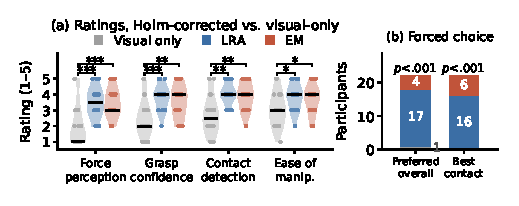
\includegraphics[width=0.8\columnwidth]{preprint_likert}
    \captionof{figure}{Participant ratings ($n=22$). (a) Ratings per item (spread, individual
      points, median), compared against vision only
      ($^{*}p<.05$, $^{**}p<.01$, $^{***}p<.001$). (b) Which condition was preferred.}
    \label{fig:likert}
  \end{center}

  \section{Discussion and Conclusion}

  Touch feedback improved fragile-object handling both in what participants did and in what
  they reported, and the recordings show why. Once the felt signal stopped growing, people
  stopped squeezing and stopped hunting for the right force. The benefit did not appear for
  deformable objects, which fits the setup, since soft objects dent the gel too little to
  give a strong signal and have no sudden breakage to avoid.

  The two actuators could not be told apart. No recorded measure separated them after
  correction, and the equivalence test reached ``close enough to be the same'' for only 3 of
  14 measure-object pairs. With 22 participants, this study could not distinguish them, not
  that they are the same. The comparison is also confounded, since they differ in technology,
  mounting position, and how well hand tracking worked. EM sits on the fingertips, partly
  covering the points the hand tracker follows, so tracking confidence dropped and thresholds
  had to be lowered. The preference for LRA may therefore reflect smoother control, not a
  better sensation.

  The largest limitation is trial order. Vision only ran first for nearly everyone, so it is
  mixed up with lack of practice, and part of the vision-versus-touch gap may just be people
  getting used to the pinch control. LRA versus EM, whose order was varied, is less exposed.
  Hand tracking is also 2D and uncalibrated, grip force is a stand-in rather than newtons,
  peak depth is capped by the safety cutoff, and the end-to-end delay still needs a bench
  measurement. Future work will mount both
  actuators in the same place, use a balanced order, calibrate against a load cell, drive the
  LRA with a dedicated chip, and send a spatial pattern rather than one number per finger.

  Overall, tactile feedback made grasping fragile objects safer, while a larger study is
  needed to tell the two actuators apart.

  \section{References}

  \begin{scriptsize}
    [1] Johansson, R. S., \& Flanagan, J. R. (2009).
    Coding and use of tactile signals from the fingertips in object
    manipulation tasks. \textit{Nat. Rev. Neurosci.}, 10(5), 345--359.
    \ [2] Pacchierotti, C., et al. (2017). Wearable haptic systems
    for the fingertip and hand. \textit{IEEE Trans. Haptics}, 10(4),
    580--600. \ [3] Lin, C., et al. (2023). 9DTact. arXiv:2308.14277.
    \ [4] Vechev, V., et al. (2019). TacTiles. \textit{IEEE VR}, 312--320.

  \end{scriptsize}

\end{multicols}

\end{document}
